% Drawing 144/05-5 -- folder 144, batch 05, archive page 92 (PDF page 93).
% Transcription: en marge gauche, un assemblage de faces quadrangulaires numérotées (côtés marqués $0$, $1$, $2$, $3$) autour d'une face centrale $r$ munie d'une flèche de rotation ; les faces voisines portent $\tau_0 r$, $\tau_1 r$, $\tau_2 r$, $\tau_3 r$.
% Kind: quadrangular faces around a central face r. Method 2 (schematic redraw from the facsimile). Status: partial.
% Notes: The central face r (rotation arrow) and its four neighbours tau_0 r, tau_1 r, tau_2 r, tau_3 r are drawn with the side numbers 0-3 that are legible; the outer ring of faces is sketched (overinked, partly overlapping on the page) and approximate; several side numbers of the outer faces are left out.
% Coordinates: 1 unit = 1 mm = 1/100 of the crop width (bbox in page fractions: [0.15, 0.37, 0.45, 0.53]).
% Redrawn by Claude (claude-opus-5-5), issue #73, 2026-11-07; not checked by a human; not compiled (no TeX in the session).
% Rights: reproduces part of the work -- behind RENDER_TRANSCRIPTS, never published by itself.
\documentclass[tikz,border=3pt]{standalone}
\usepackage{amsmath,amssymb}
\usetikzlibrary{patterns,arrows.meta}
\tikzset{pencil/.style={black!45}, struck/.style={black!35}, mark/.style={circle,draw,inner sep=1.3pt}, pt/.style={circle,fill,inner sep=0.9pt}, opt/.style={circle,draw,fill=white,inner sep=1.1pt}}
\begin{document}
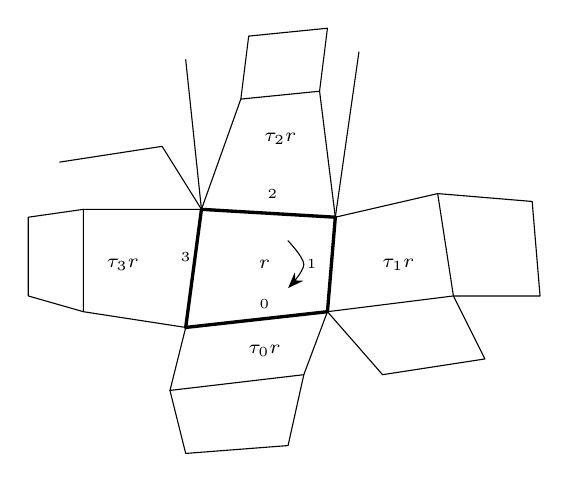
\begin{tikzpicture}[x=1mm,y=1mm,line cap=round,line join=round,font=\scriptsize]
\draw[very thick] (32,-41) -- (49,-42) -- (48,-54) -- (30,-56) -- cycle;
\draw (32,-41) -- (37,-27) -- (47,-26) -- (49,-42);
\draw (49,-42) -- (62,-39) -- (64,-52) -- (48,-54);
\draw (30,-56) -- (28,-64) -- (45,-62) -- (48,-54);
\draw (32,-41) -- (17,-41) -- (17,-54) -- (30,-56);
\draw (37,-27) -- (38,-19) -- (48,-18) -- (47,-26);
\draw (62,-39) -- (74,-40) -- (75,-52) -- (64,-52);
\draw (17,-41) -- (10,-42) -- (10,-52) -- (17,-54);
\draw (14,-35) -- (27,-33) -- (32,-41);
\draw (30,-22) -- (32,-41);
\draw (52,-21) -- (49,-42);
\draw (48,-54) -- (55,-62) -- (68,-60) -- (64,-52);
\draw (28,-64) -- (30,-72) -- (43,-71) -- (45,-62);
\node[inner sep=1pt] at (41,-39) {\tiny $2$};
\node[inner sep=1pt] at (46,-48) {\tiny $1$};
\node[inner sep=1pt] at (40,-53) {\tiny $0$};
\node[inner sep=1pt] at (30,-47) {\tiny $3$};
\node[inner sep=1pt] at (40,-48) {\scriptsize $r$};
\draw[-{Stealth[length=2mm]}] plot[smooth, tension=0.55] coordinates {(43,-45) (45,-48) (43,-51)};
\node[inner sep=1pt] at (42,-32) {\scriptsize $\tau_2 r$};
\node[inner sep=1pt] at (57,-48) {\scriptsize $\tau_1 r$};
\node[inner sep=1pt] at (40,-59) {\scriptsize $\tau_0 r$};
\node[inner sep=1pt] at (22,-48) {\scriptsize $\tau_3 r$};
\end{tikzpicture}
\end{document}
